\chapter{Orchestration des applications distribuées}
\begin{onehalfspace}

\initial{D}ocker est un outil qui a révolutionné le monde informatique par l'introduction de la notion de container, donc il est normal de chercher  à l'utiliser en production. De nos jours, les développeurs utilisent de plus en plus Docker pour déployer des applications qui s'éxecutent sur plusieurs conteneurs et plusieurs hôtes. Orchestrer ces applications distribuées nécessite une approche \textbf{multi-conteneur} et \textbf{multi-hôte} native avec une interface utilisateur et de l'outillage commun qui fonctionne sur toutes les infrastructures. Plusieurs outils ont été présentés par de grandes entreprises et sont toujours en cours de développement. Nous exposerons dans ce chapitre les projets promoteurs dans l'orchestration des applications distribuées.

\newpage

\section{Le clustering}

Nous avons présenté dans le chapitre 2 le Cloud Computing ainsi que les services classiques que l'on peut trouver. Dans cette section, nous allons parler du cluster comme service et l'on va le situer dans le pyramide des services du Cloud (Figure ~\ref{fig:pyramide-cluster}, page~\pageref{fig:pyramide-cluster}).

\begin{figure}[H]
\centering
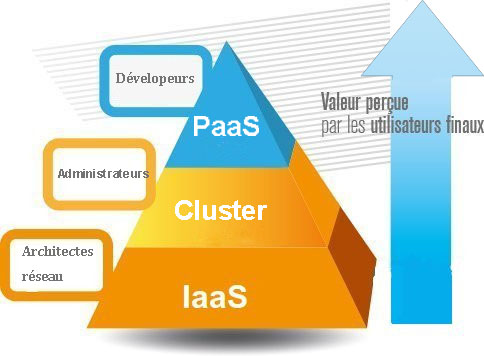
\includegraphics [scale=0.7]{chapitre3/assets/pyramide}
\caption{Le cluster dans le cloud}
\label{fig:pyramide-cluster}
\end{figure}

\begin{itemize}
	\item \textbf{Plate-forme}: On développe une application dans un ensemble particulier de langages de programmation à l'aide d'un ensemble particulier des \acrshort{api}s et l'on pousse ce code vers la plate-forme. La plate-forme exécute et lance une seule copie ou éventuellement plusieurs copies de celui-ci dépendemment du traffic, il monte en charge automatiquement. 
	\item \textbf{\acrshort{iaas}}: A l'autre bout du pyramide, on trouve l'\acrshort{iaas}, seulement des machines virtuelles, donc ce sont des ordinateurs ordinaires, sauf qu'ils vivent essentiellement dans l'internet. Quand on va chez un fournisseur \acrshort{iaas} et l'on demande de nous fournir un ordinateur avec une telle quantité de mémoire et de disque, un tel nombre de \acrshort{cpu} et qui exécute une version spécifique de Linux; dans quelques secondes on a notre ordinateur où l'on peut exécuter n'importe quel logiciel, mais on est responsable de la gestion de la machine entière.
	\item \textbf{Cluster}: C'est lorsque l'on veut gérer un ensemble de machines, un cluster de machines comme une seule entité, pas seulement un ordinateur individuel (\acrshort{iaas}) et pas toute une plate-forme magique parce que l'on veut faire plus. C'est une question d'agilité et de la flexibilité.

\end{itemize}


\def\arraystretch{1.6}%  1 is the default, change whatever you need

{\rowcolors{1}{tabOdd}{tabEven}
\begin{center}
\begin{table}[H]

	\caption{Le cluster dans le cloud \label{tab:table_label}}
	\begin{tabu}{| X[c] | X[c] | X[c] | X[c] |} 


	\hline
	\rowcolor{tabHead}
	\textbf{} & \textbf{IaaS (VMs)} & \textbf{Cluster} & \textbf{Plate-forme}\\ [0.95ex] 
	\hline\hline
	A quoi sert ? 	& Créer et déployer les images des machines virtuels & Créer et déployer des conteneurs & créer et déployer des applications (services) \\ 
	Automatise					& - & Ordonnancement & Tout \\ 
	gére					& Un seul atome & Des serveurs & Des applications \\ 
	fléxibilité					& ++ 	& + 	& - \\ 
	Agilité						& - 	& + 	& ++ \\ 
	\hline
	\end{tabu}
\end{table}
\end{center}
}


\begin{itemize}
	\item Master: C'est la machine qui est responsable du cluster. Il veille sur son bon fonctionnement grâce au système de découverte des services et l'ordonnanceur
	\item Ordonnanceur: Dans un ordinateur ordinaire, pour démarrer un processus, on a besoin d'un gestionnaire des processus pour les faire fonctionner et les garder en cours d'exécution. L'ordonnanceur le fera sur l'ensemble des machines (cluster)
	\item Noeud: Une machine qui appartient au cluster, elle peut être réel ou virtuel
	\item Gestionnaire des conteneurs: C'est la partie de logiciel qui est distribué dans chaque machine du cluster. Il supervise les conteneurs ordonnancés, les redémarre en cas de nécéssité...
	\item Conteneurs ordonnancés: Un service fonctionne à l'intérieur d'un conteneur ordonnancé. En effet, ce conteneur ne s'est pas trouvé dans une telle machine par hasard ou suivant la volonté du développeur, mais parce que le développeur a déclaré à l'ordonnanceur de cluster, le maître, que le service a besoin, par exemple, d'exécuter dix copies de ce service, 3 coeurs, 2 Go de mémoire et peu de disque. L'ordonnanceur fournit pour le service un endroit où il peut vivre en paix.
\end{itemize}


\begin{figure}[H]
\centering
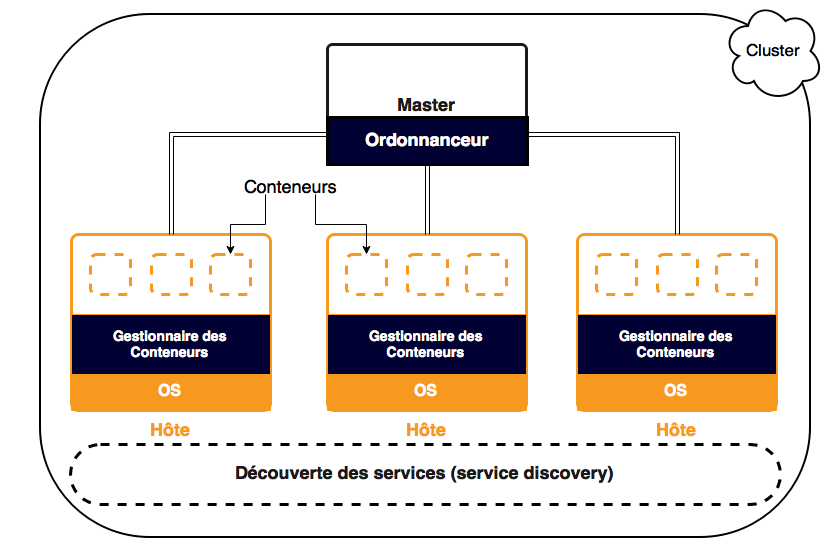
\includegraphics [scale=0.55]{chapitre3/assets/cluster}
\caption{Un cluster en général}
\label{fig:}
\end{figure}

Nous avons vu la notion de cluster et les processus d'automatisation, d'organisation, de coordination, et de gestion de services informatiques distribués incontournables à son fonctionnement, c'est ce que l'on appelle \textbf{l'orchestration}. Dans la section suivante, nous allons détailler les différents solutions d'orchestration qui existent dans le monde de containérisation (Docker).

\section{Orchestration Docker}
Les capacités d'orchestration de Docker sont construites sur les fondations de l'engine Docker existante. Ces capacités sont assurées par trois nouveaux services de la plate-forme qui sont conçus pour couvrir tous les aspects du cycle de vie dynamique des applications distribuées. Selon l'entreprise Docker, toutes ces caractéristiques sont conçues avec la philosophie de conception "\emph{Batteries Included, but Removable}" qui indique qu'ils peuvent fonctionner avec des services tierces. Ceci offre le choix aux clients de choisir entre les différents outils d'orchestration de Docker et les alternatives communautaires.


%\begin{figure}[H]
%\centering
%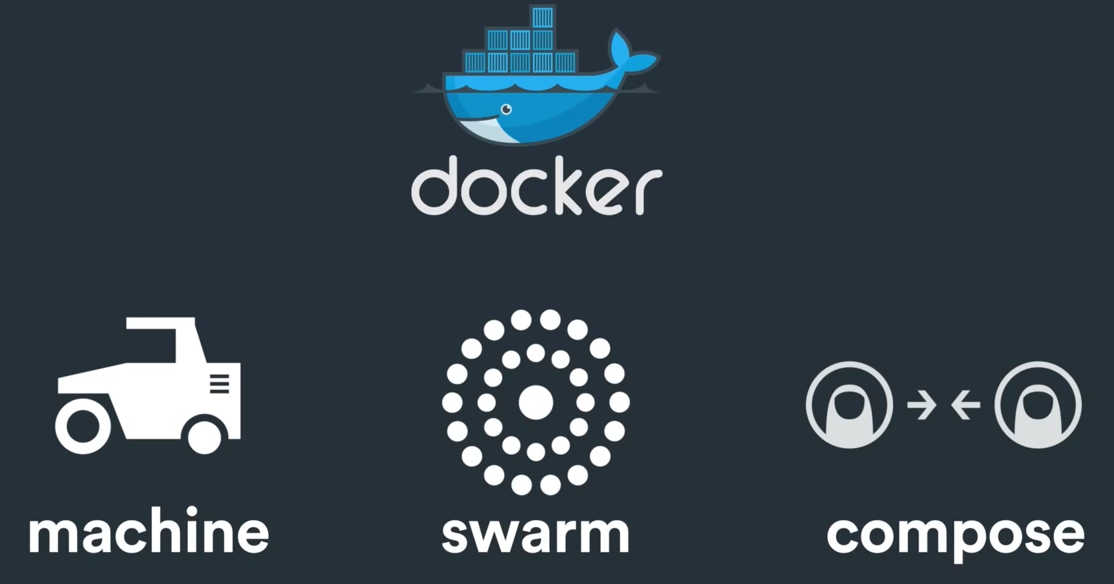
\includegraphics [scale=0.4]{chapitre3/assets/orchestrationdocker.png}
%\caption{Orchestration Docker}
%\end{figure}
\subsection{Docker Machine}
 Ce service facilite le provisionning d'un hôte avec Docker installé dans une variété d'environnements. Les développeurs peuvent rapidement lancer les machines hôtes exécutant Docker ; sur un ordinateur portable, un datacenter de VMs, ou une instance Cloud. Cela évite la tâche de se connecter à un hôte pour installer et configurer le démon Docker et le client. Bien que toujours en version alpha, Docker machine prend en charge le provisionning de Docker localement avec VirtualBox et à distance sur les instances Digital Ocean. Le support pour AWS, Azure, VMware, OpenStack et d'autres infrastructures devrait arriver rapidement.
 \begin{figure}[H]
\centering
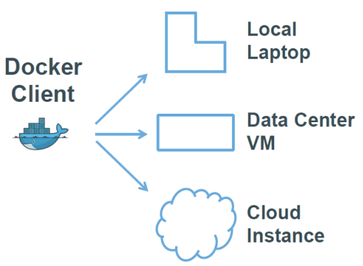
\includegraphics [scale=0.6]{chapitre3/assets/dockermachine.png}
\caption{Docker Machine}
\end{figure}
\subsection{Docker Swarm}
 Docker Swarm est un service de clustering natif de Docker qui fonctionne avec l'engine Docker standard, et qui crée un pool de ressources, les hôtes, sur lesquels les applications distribuées s'exécutent. Cela permet aux développeurs et aux équipes opérationnelles de considérer un cluster de machines Docker comme un pool de ressources unique. Les administrateurs peuvent planifier des conteneurs qui seront lancés dans l'un des hôtes qui répond aux exigences. Docker Swarm fournit des contraintes standard et personnalisées pour répondre aux besoins et à la planification basée sur des règles. Cela permet aux administrateurs de déclarer des exigences et contraintes spécifiques à chaque conteneur. Docker Swarm est conçu pour évoluer avec le cycle de vie de l'application. Il peut prendre en charge d'un hôte dans l'environnement de développement à des centaines s'exécutant dans l'environnement de production.
\begin{figure}[H]
\centering
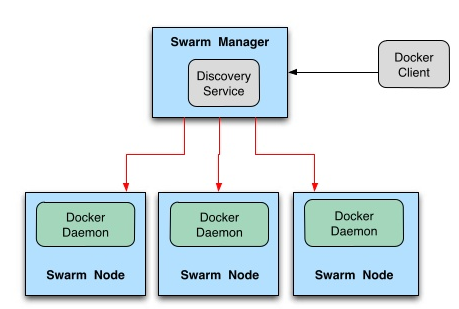
\includegraphics [scale=0.6]{chapitre3/assets/dockerswarm.png}
\caption{Architecture de Docker Swarm}
\end{figure}
\subsection{Docker Compose}
  Docker Composer permet aux développeurs d'assembler des applications de conteneurs Docker autonomes et interopérables et indépendantes de l'infrastructure sous-jacente. Avec cette approche déclarative, il est facile de définir des stacks qui sont portables. Une stack d'applications distribuées est déclarée à travers un simple fichier de configuration \acrshort{yaml} qui contient la définition de chaque conteneur.
\begin{figure}[H]
\centering
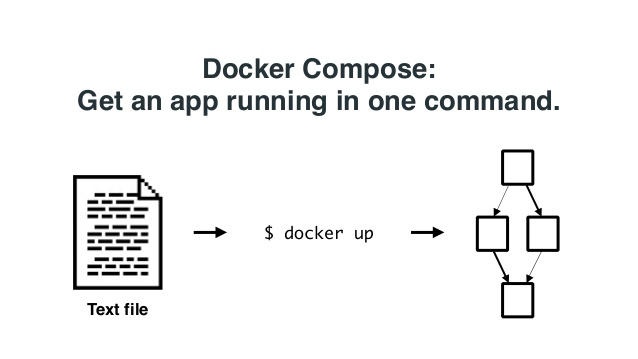
\includegraphics [scale=0.5]{chapitre3/assets/dockercompose.jpg}
\caption{Docker Compose}
\end{figure}
\section{Orchestration Google}
L'entreprise Google est aussi interessée par l'orchestration des conteneurs docker, elle a d'ailleurs lancée un projet nommée \textbf{Kubernetes}.Ce projet est récent mais très promoteur et pourrait révolutionner le domaine du Cloud s'il est suffisament mature pour la production. Kubernetes a pour objectif de fournir un outil de supervision unique capable de déplacer des conteneurs Docker d'un cloud à un autre. Autrement dit, de proposer une forme d’interopérabilité dans le nuage, via un framework de gestion des conteneurs solide, ouvert et adapté à toute application sur tous types d’environnements, qu’il s’agisse de Cloud privé, public ou hybride. Ce projet a le soutien et l'attention des géants du cloud notamment Microsoft, IBM, RedHat qui tiennent à s'assurer que cet outil sera compatible avec leurs clouds et l'associer au projet \textbf{Openstack} qui est l'orchestrateur du cloud hybride open source.
\subsection{Architecture de Kubernetes}
Kubernetes est un outil open-source pour l'orchestration des conteneurs Docker. Il gère l'ordonnancement des noeuds dans un \textbf{cluster} et gère les ressources pour mieux correspondre à l'intention de l'utilisateur. En Utilisant les concepts de "\emph{labels}" et "\emph{pods}", il permet un regroupement optimal des conteneurs pour une meilleure gestion et une découverte facile.
\begin{figure}[H]
\centering
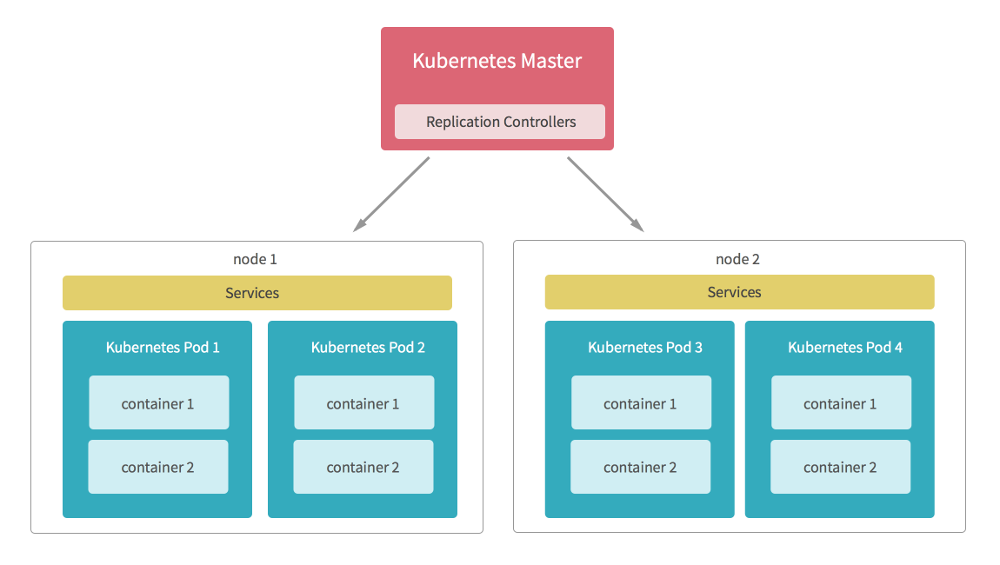
\includegraphics [scale=0.5]{chapitre3/assets/archkuber.png}
\caption{Architecture de Kubernetes}
\end{figure}

\begin{itemize}
\item \textbf{Kubernetes Master} : Il contrôle l'ensemble du cluster et exécute l'API pour le cluster. Fondamentalement, il est responsable du cluster.

\item \textbf{Nodes} : Un nœud est un serveur physique (ou une machine virtuelle ) à l'intérieur du cluster. Il communique avec les maîtres et contient des conteneurs, on peut ajouter ou supprimer des noeuds à volonté.

\item \textbf{Pods} : Un "Pod" est le bloque basique de construction dans \emph{Kubernetes}.Dans un pod, il est possible de lancer plusieurs conteneurs. L'allocation des CPU, mémoire et des autres ressources est gérée dans un pod. Chaque pod possède sa propre adresse ip et son nom d'hôte pour éviter d'éventuels conflicts de ports.

\item \textbf{Replication Controller} : Il est vrai que le Pod est un composant puissant au sein de \emph{Kubernetes} mais il ne permet pas la gestion des échecs. Les échecs sont des événements inévitables bien qu'il faudrait que le service soit toujours disponible. c'est de ce fait qu'intervient \emph{Replication Controller}. Ce dernier s'assure qu'un nombre donné de pods sont exécutés au sein du cluster , il peut enlever et ajouter des pods du cluster donc il faudra définir un pod template pour assurer sa fonction.

\item \textbf{Services} : les Pods sont ajoutés ou supprimés donc il faudrait permettre un \textbf{load-balancing} du traffic dans ses pods. "\emph{Service}" agit comme un \emph{load-balancer} dynamique pour un ensemble de pods, il est très efficace et utilise différentes techniques ( IP Tables, ...) pour éviter la surchage.

\end{itemize}
\begin{figure}[H]
\centering
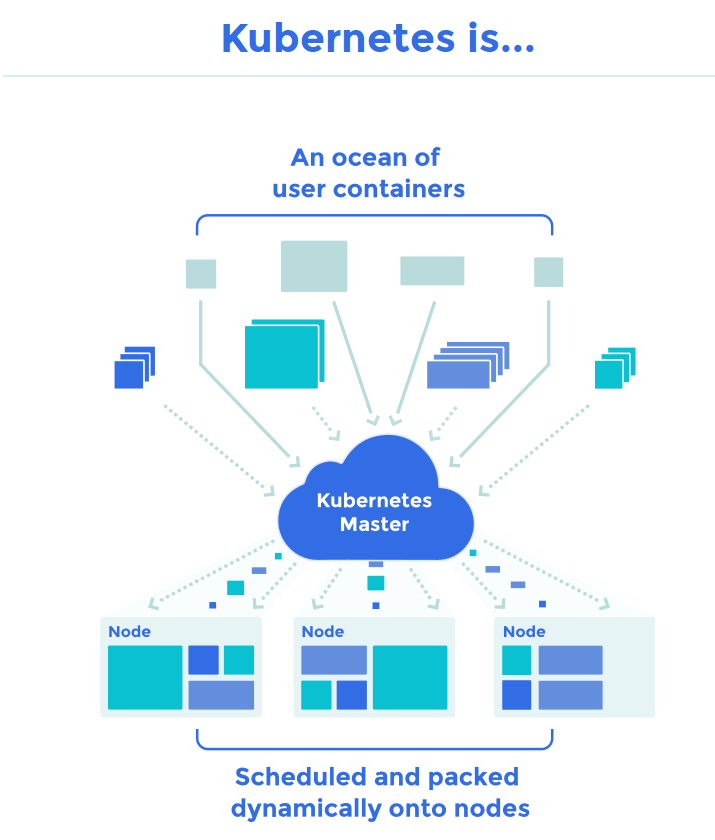
\includegraphics [scale=0.5]{chapitre3/assets/kuber.png}
\caption{Résumé de Kubernetes}
\end{figure}

\section{Orchestration Apache}
L'entreprise Apache a toujours été intéressée par le domaine du Cloud, le lancement de son projet \textbf{Mesos} visait principalement à améliorer l'orchestration des \emph{"datacenters"} ceci bien avant l'emergence des conteneurs et docker. Le projet Mesos est très promoteur pour le futur avec les conteneurs bien qu'il soit déjà mature avec les machines virtuelles. Plusieurs grandes entreprise utilisent Mesos notamment \emph{Twitter}, \emph{Paypal} et \emph{Airbnb}.
Mesos agit comme un "Cluster Manager" et offre de nombreuses fonctionnalités telles que :
\begin{itemize}
\item Une scalabilité à plus de 10000 noeuds.
\item Isolement des ressources pour les tâches via les conteneurs linux (LXC).
\item Gestion efficace du CPU et de la mémoire interne.
\item Haute disponibilité du master via Apache Zookeeper.
\item Une interface Web pour le monitoring des clusters.
\end{itemize}
\subsection{Architecture de Mesos}
\emph{Mesos} possède une architecture composée principalement de maîtres, esclaves et "Frameworks". Nous définirons dans cette partie les composants pertinents de l'architecture suivante.
\begin{figure}[H]
\centering
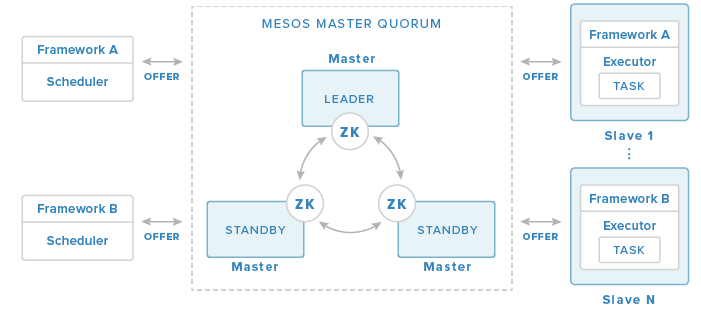
\includegraphics [scale=0.65]{chapitre3/assets/mesosarch.png}
\caption{Architecture de Mesos}
\end{figure}
\begin{itemize}
\item \textbf{Master daemon} : Il tourne dans noeud "master" et gère les esclaves.
\item \textbf{Slave daemon} : Il tourne aussi dans un noeud "master" et exécute les tâches des "Frameworks".
\item \textbf{Framework} : connu aussi par l'application Mesos, il est composé d'un ordonnaceur qui gère les offres d'allocation de ressources, et d'un ou plusieurs "executors" qui lancent les tâches sur les esclaves.
\item \textbf{Offer} : C'est une liste des ressources disponibles de la mémoire et du CPU propre à un noeud esclave. Tous les noeuds esclaves envoient des offres pour le maître  et ce dernier transmet ces offres aux "frameworks" disponibles.
\item  \textbf{Task} : c'est un tâche qui est ordonnancée par un "framework" et qui est exécutée dans un noeud esclave. Cette tâche peut être de n'importe quel type (commande, script bash ,requête SQL, Hadoop Job, ...)
\item \textbf{Apache ZooKeeper }: C'est un logiciel qui coordonne les noeuds maîtres.
\end{itemize}
\subsection{Frameworks Mesos}
Le framework ou l'application Mesos tient une importante place au sein de l'architecture. Dans cette partie , on présentera 2 importants frameworks qui sont \textbf{Marathon} et \textbf{Chronos}.
\begin{figure}[H]
\centering
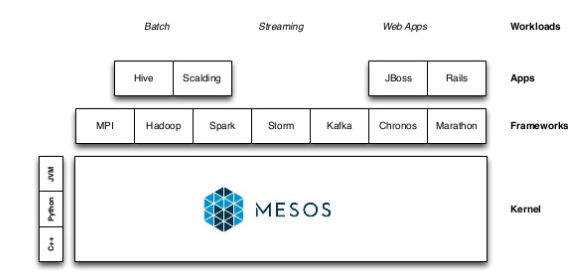
\includegraphics [scale=0.65]{chapitre3/assets/framework.png}
\caption{Composants de l'architecture Mesos}
\end{figure}
\subsubsection{Marathon}
\emph{Marathon} est un framework Mesos développé pour éxécuté les applications "\emph{long-running}". Il sert de remplacement pour le système \emph{init}. Il possède de nombreuses fonctionnalités qui simplifient les applications en cours d'exécution dans un environnement en cluster telles que la haute disponibilité, les contraintes de nœuds, des contrôles de santé de l'application, une API pour scriptabilité et la découverte de service et un outil facile à utiliser l'interface utilisateur Web UI. Il ajoute ses capacités de mise à l'échelle et d'auto- guérison de l'ensemble des fonctionnalités de Mesos. 
\subsubsection{Chronos}
\emph{Chronos} est une application Mesos qui a été initialement développé par Airbnb comme remplacement pour le système \emph{cron}.Il est un ordonnanceur pleinement fonctionnel , distribué et tolérant aux pannes pour \emph{Mesos}, ce qui facilite l'orchestration des "\emph{jobs}" qui sont des collections de tâches . Il comprend une API qui permet d'exécuter les scripts de la planification de tâches et une interface web pour la facilité d'utilisation.
\emph{Chronos} est complémentaire à \emph{Marathon} car il fournit une autre façon d'exécuter des applications selon un calendrier ou d'autres conditions telles que la réalisationn d'un autre emploi. Il est également capable de la planification de tâches sur plusieurs noeuds esclaves Mesos, et fournit des statistiques sur les échecs et les réussites d'emploi.

   
 

\end{onehalfspace}